\documentclass[landscape]{article}
\usepackage{graphicx}
\usepackage{subfig}
\usepackage[top=0.4in,bottom=0.4in,left=0.75in,right=0.5in]{geometry}
\DeclareGraphicsExtensions{.pdf}
\usepackage{nopageno}
\pagestyle{plain}
\usepackage{array}
\usepackage[export]{adjustbox}
\usepackage{booktabs} % table features
\usepackage[abs]{overpic} % overlaying one graphic on another
\usepackage{xstring,xifthen} % string length with conditionals
\usepackage{color} % colored text
%\usepackage{helvet} % font

%\usepackage{cmbright} % font

\renewcommand{\familydefault}{\sfdefault}


%\topmargin -1.2in

\parindent=0pt
\baselineskip=0pt
\parskip=0pt

\input{macros.tex}
\def\yourname{Your Name Here}

%\usepackage{unicode-math}
%\setmainfont[
%   UprightFont = * Condensed Medium,
%      BoldFont = * Medium,
%    ItalicFont = * Condensed Medium,
%%    ItalicFont = * Medium Italic,
%]{Futura}



\begin{document}

\begin{tabular}{ @{} m{4.05cm} m{16cm} }
	
\includegraphics[height=0.08\textheight]{pdfs/logoshape.pdf} & 
\includegraphics[height=0.06\textheight]{pdfs/headerbw.pdf} \\
\end{tabular}
	
\vspace{0.65cm}

\begin{center}

\StrLen{\yourname}[\yournameLen]

\ifthenelse{\yournameLen < 28}{
	{\fontsize{40}{50}\selectfont {\MakeUppercase {\bf \yourname}}}
}{
	{\fontsize{36}{50}\selectfont {\MakeUppercase {\bf \yourname}}}
}

\end{center}

\vspace{0.65cm}

{\Huge What's in your American Gut?}

\vspace{2mm}

\begin{tabular*}{\textwidth}{ m{3.2in} m{7.7in} }
	\vspace{-2mm}
    \hspace{0mm}
    \begin{overpic}[width= 2.10in]{pdfs/figure4.pdf}
		\put(-32,-39){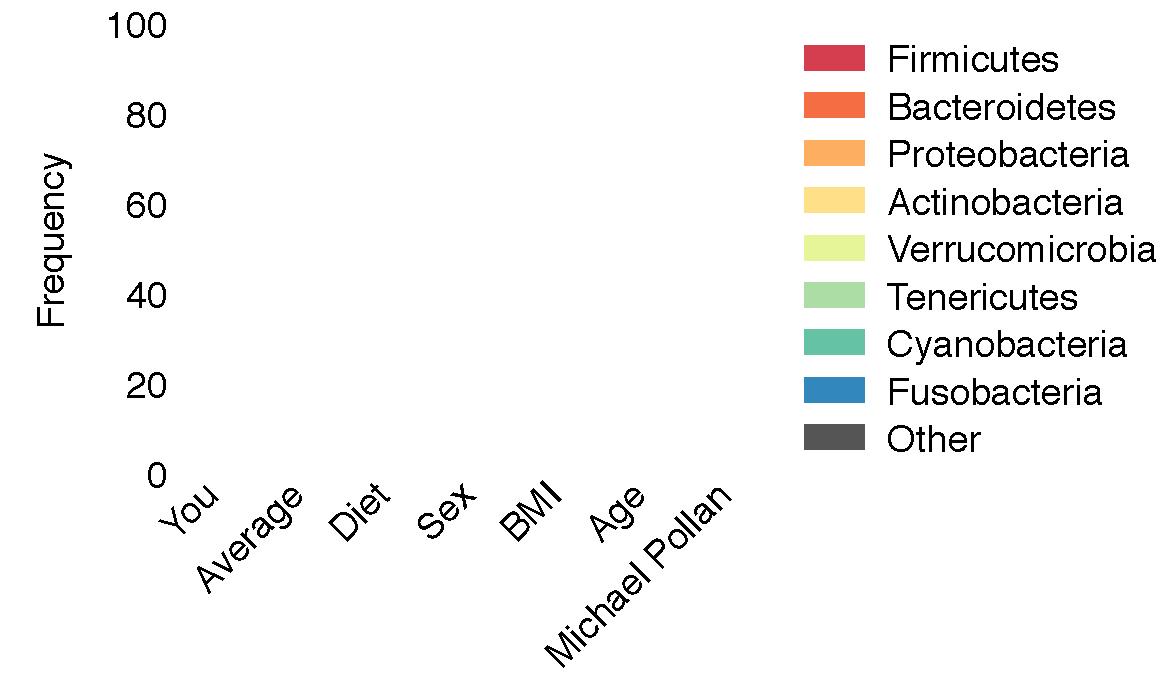
\includegraphics[width=3.65in]{pdfs/figure4_overlay.pdf}}
	\end{overpic} 
    &
    {\normalsize 
    \vspace{5mm}
    \parbox[b][][t]{6.5in}{
	\begin{tabular}{ c l r c l r r r }
    	    \multicolumn{3}{l}{\large Your most abundant microbes:} & \multicolumn{5}{l}{\large Your most enriched microbes:}\\ \addlinespace[2mm]
		\cline{2-3} \cline{5-8} \addlinespace[1mm]
		& Taxonomy & Sample & & Taxonomy & Sample & Population & Fold \\
		\cline{2-3} \cline{5-8} \addlinespace[1mm]
		& \abundTaxonA{} & \abundSamplA{}\% & & \enrichTaxonA{} & \enrichSamplA{}\% & \enrichPopulA{}\% & \enrichFolddA{}x \\
		& \abundTaxonB{} & \abundSamplB{}\% & & \enrichTaxonB{} & \enrichSamplB{}\% & \enrichPopulB{}\% & \enrichFolddB{}x \\
		& \abundTaxonC{} & \abundSamplC{}\% & & \enrichTaxonC{} & \enrichSamplC{}\% & \enrichPopulC{}\% & \enrichFolddC{}x \\
		& \abundTaxonD{} & \abundSamplD{}\% & & \enrichTaxonD{} & \enrichSamplD{}\% & \enrichPopulD{}\% & \enrichFolddD{}x \\
		\cline{2-3} \cline{5-8} \addlinespace[3mm]
		& \multicolumn{7}{p{5.6in}}{\normalsize \rareList{}.}
	\end{tabular}
	}
	}
\end{tabular*}

\vspace{1.4cm}

{\Huge How do your gut microbes compare to others?} 
%\begin{overpic}
%	\put(0.0){
\includegraphics[width=0.75in]{pdfs/ball_legend.pdf}}
%\end{overpic}

\vspace{0mm}

\begin{figure}[!ht]

\raisebox{29mm}{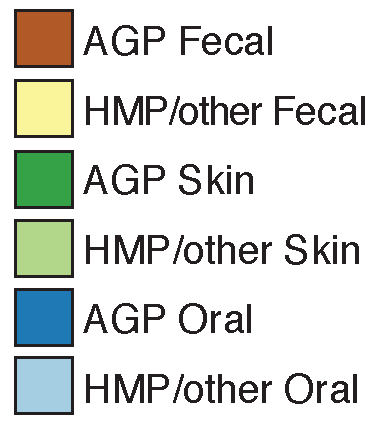
\includegraphics[scale=0.40]{pdfs/figure1_legend.pdf}}
\hspace{-10mm}
\subfloat[Different body sites\label{subfig-1:dummy}]{%
\begin{overpic}[height=0.30\textheight]{pdfs/figure1.pdf}
	\put(0,-5){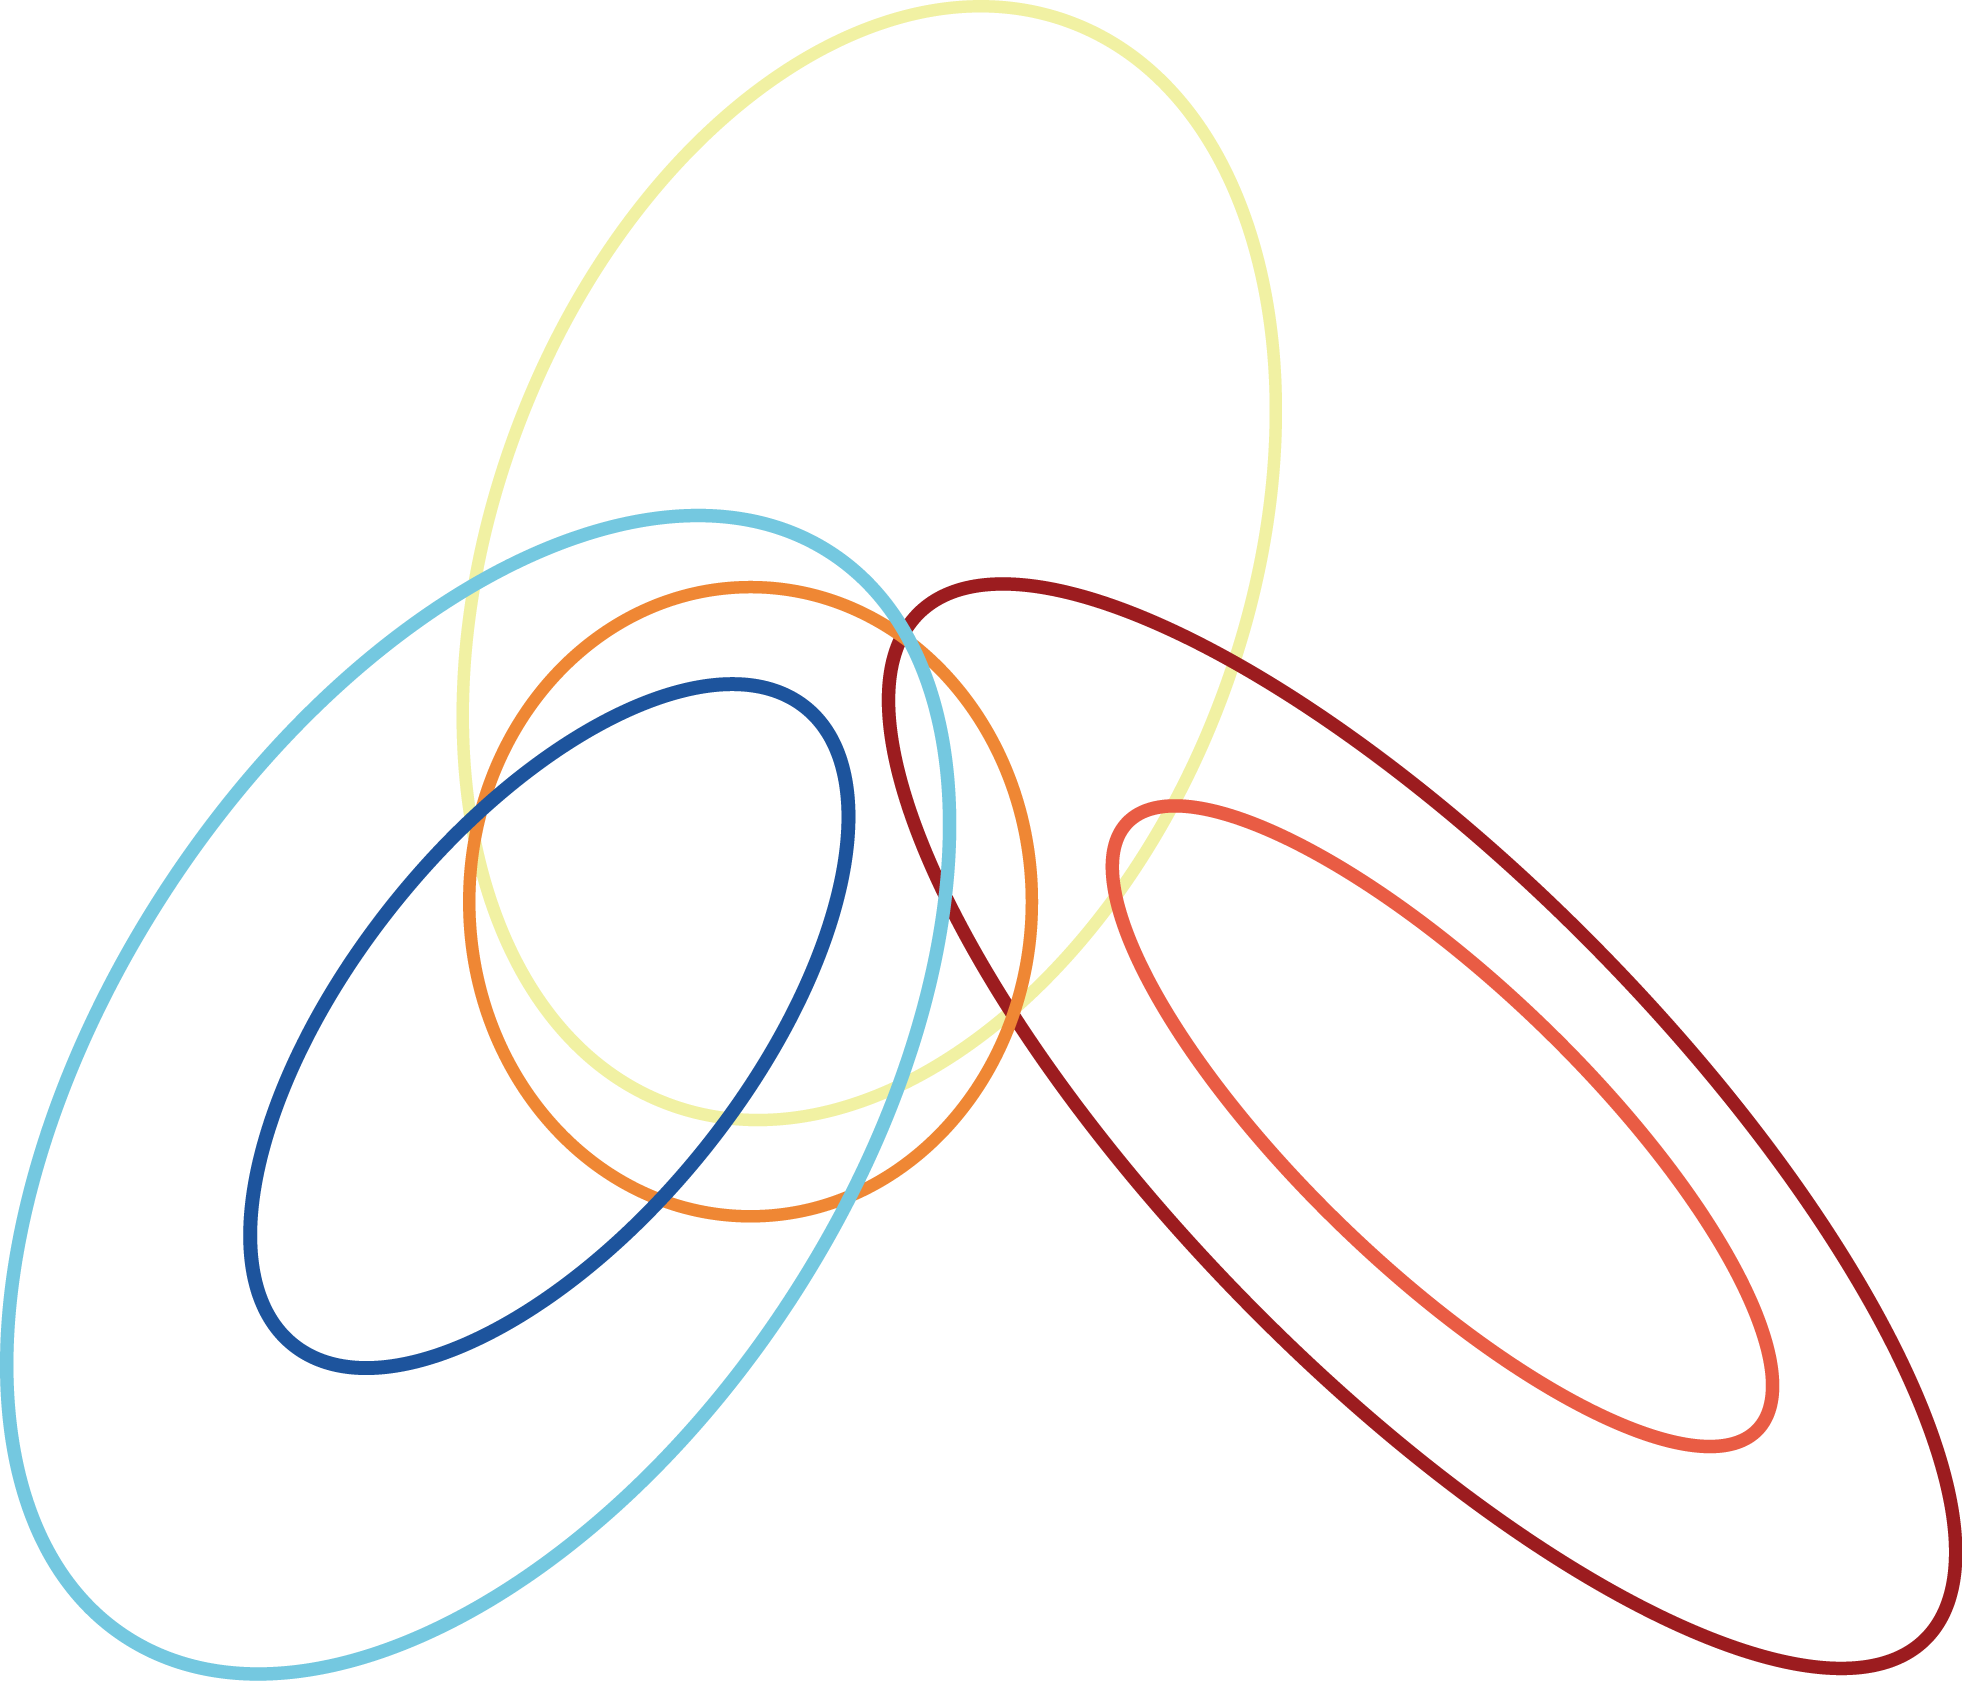
\includegraphics[scale=0.40]{pdfs/figure1_ovals.png}}
\end{overpic}
}
%
\hspace{0mm}
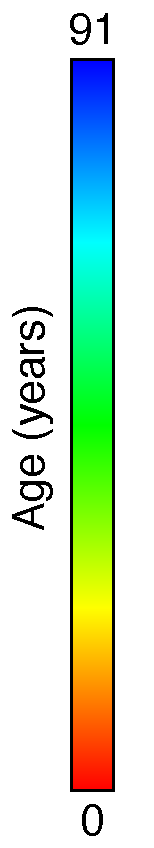
\includegraphics[scale=0.40]{pdfs/figure2_legend.pdf}
\subfloat[Different ages and populations\label{subfig-2:dummy}]{%
\begin{overpic}[height=0.30\textheight]{pdfs/figure2.pdf}
	\put(0,0){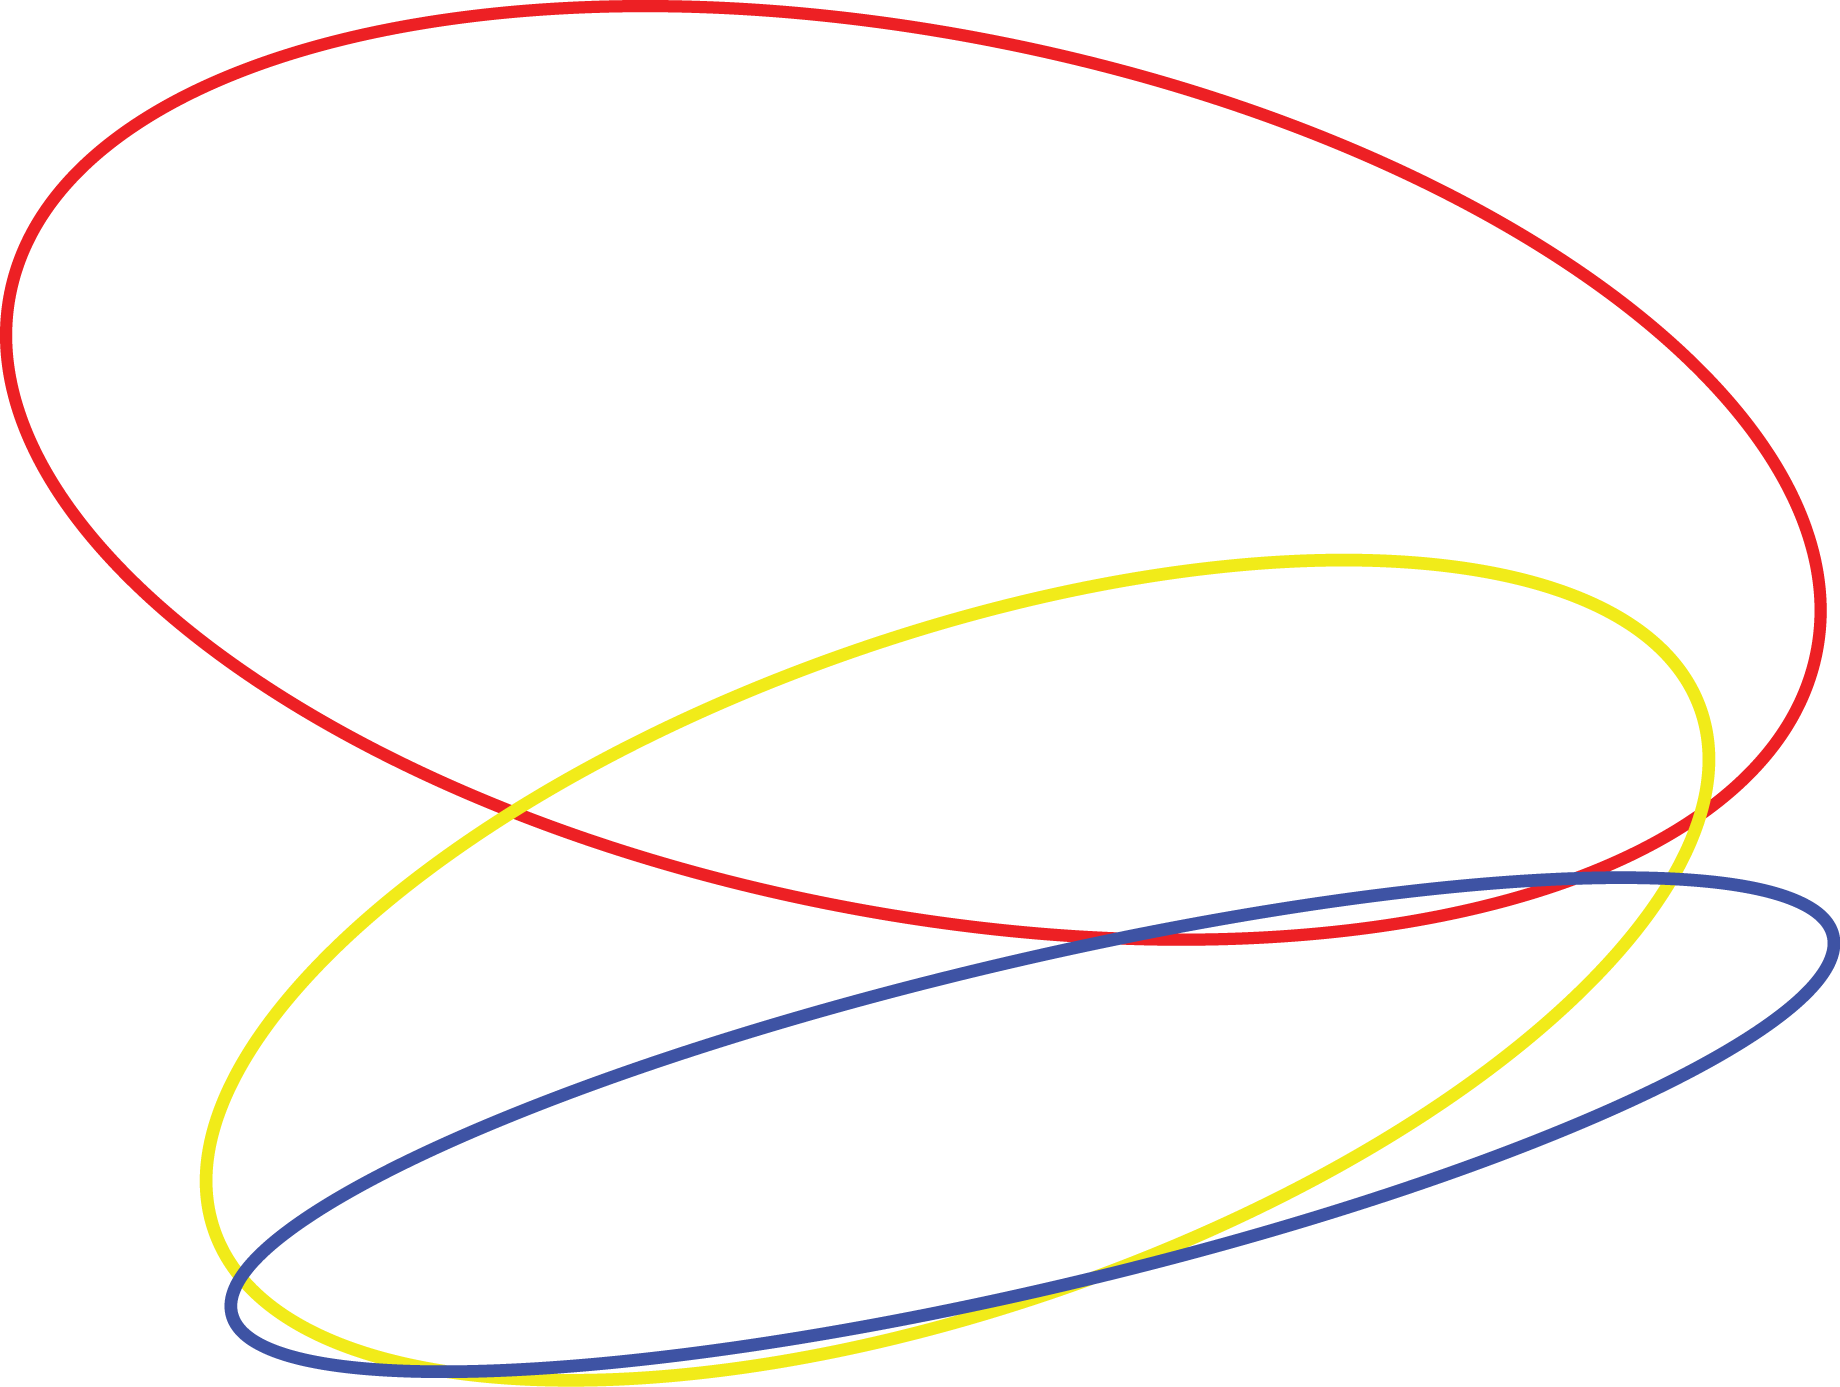
\includegraphics[scale=0.48]{pdfs/figure2_ovals.png}}
	\put(165,0){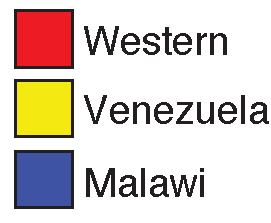
\includegraphics[scale=0.40]{pdfs/figure2_country_legend.pdf}}
 	\put(190,140){
\includegraphics[scale=0.45]{pdfs/ball_legend.pdf}}
\end{overpic}
}
%
\hspace{8mm}
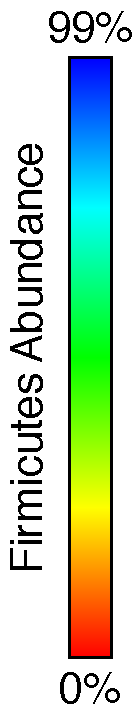
\includegraphics[scale=0.40]{pdfs/figure3_legend.pdf}
\subfloat[The American Gut population\label{subfig-3:dummy}]{%
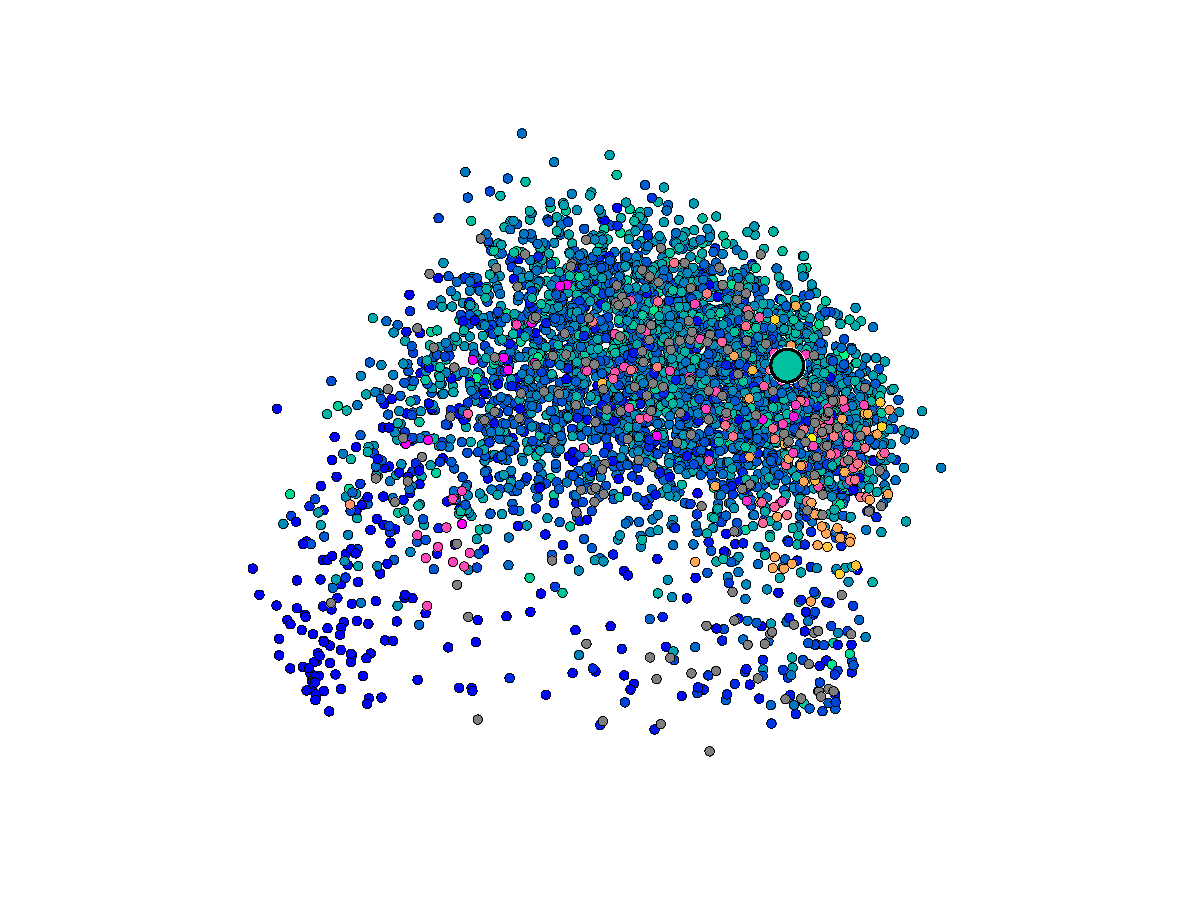
\includegraphics[height=0.30\textheight]{pdfs/figure3.pdf}
}
\end{figure}



\end{document}

